%%%%%%%%%%%%%%%%%%%%%%%%%%%%%%%%%%%%%%%%%
%  My documentation report
%  Objetive: Explain what I did and how, so someone can continue with the investigation
%
% Important note:
% Chapter heading images should have a 2:1 width:height ratio,
% e.g. 920px width and 460px height.
%
%%%%%%%%%%%%%%%%%%%%%%%%%%%%%%%%%%%%%%%%%

%----------------------------------------------------------------------------------------
%	PACKAGES AND OTHER DOCUMENT CONFIGURATIONS
%----------------------------------------------------------------------------------------

\documentclass[11pt,fleqn]{book} % Default font size and left-justified equations

\usepackage[top=3cm,bottom=3cm,left=3.2cm,right=3.2cm,headsep=10pt,letterpaper]{geometry} % Page margins
\usepackage[dvipsnames]{xcolor}
\usepackage{lipsum} % Required for specifying colors by name

% Font Settings
\usepackage{avant} % Use the Avantgarde font for headings
%\usepackage{times} % Use the Times font for headings
\usepackage{mathptmx} % Use the Adobe Times Roman as the default text font together with math symbols from the Symbol, Chancery and Computer Modern fonts

\usepackage{microtype} % Slightly tweak font spacing for aesthetics
\usepackage[utf8]{inputenc} % Required for including letters with accents
\usepackage[T1]{fontenc} % Use 8-bit encoding that has 256 glyphs

%-------- LANGUAGE ------
\usepackage{ifthen}

\provideboolean{lfrench}\setboolean{lfrench}{false} 
\provideboolean{lenglish}\setboolean{lenglish}{false} 

%\setboolean{lfrench}{true} %FRANCAIS
\setboolean{lenglish}{true} % ENGLISH

\ifthenelse{\boolean{lfrench}}{
\usepackage[french]{varioref}
\usepackage[french]{babel}
}{}

\ifthenelse{\boolean{lenglish}}{
\usepackage[english]{varioref}
%\usepackage[english]{babel}
}{}

% ------------------
\usepackage{wrapfig}
\usepackage{listings}
\usepackage{multicol}
\usepackage{multirow}
\usepackage{colortbl}
\usepackage{booktabs}
\newcommand{\tabitem}{~~\llap{\textbullet}~~}
\usepackage[backpage=page]{hyperref}
\usepackage{qrcode}
\usepackage{soul}
\usepackage{tabto}
\usepackage{multienum}

\definecolor{deepblue}{rgb}{0.0,0.0,0.5}
\definecolor{deepred}{rgb}{0.6,0,0}
\definecolor{deepgreen}{rgb}{0,0.5,0}
\definecolor{ocre}{RGB}{51,102,0} 
\definecolor{lightgray}{RGB}{229,229,229} 
\definecolor{palerod}{RGB}{238,232,170}
\definecolor{verttelecom}{RGB}{171,180,0}

\newcommand\pythonstyle{\lstset{
language=Python,
basicstyle=\ttfamily\footnotesize,
morekeywords={self},              % Add keywords here
frame=tb,                         % Any extra options here
showstringspaces=false
}}

\definecolor{backcolour}{rgb}{0.95,0.95,0.92}

\newcommand\termctyle{\lstset{
frame=tb,                         % Any extra options here
showstringspaces=false
}}


% Python environment
\lstnewenvironment{python}[1][]
{
\pythonstyle
\lstset{#1}
}
{}

\lstnewenvironment{termc}[1][]
{
\lstset{#1}
}
{}


% RFC
\newcommand\rfc[1]{\href{http://www.ietf.org/rfc/rfc#1.txt}{\textcolor{blue}{RFC #1}\index{RFC #1}}}
\newcommand\pfunction[2]{\texttt{#2}\index{Module Python!#1!#2}}

% boot.py

\newcommand\glos[1]{\gls{#1}\index{#1}}
\newcommand\pprog[2]{\href{https://github.com/ltn22/PLIDObis/blob/master/#2/#1}{\texttt{#1}}\index{Programmes Python!#1}}
\newcommand\lprog[2]{\href{https://github.com/ltn22/PLIDObis/blob/master/#2/#1}{\texttt{#1}}\index{Programmes micro-python!#1}}

% QUESTION

\usepackage[most]{tcolorbox}

\provideboolean{Response}\setboolean{Response}{true}

\newcommand{\Correct}[1]{\ifthenelse{\boolean{Response}}{#1}{\textbf{#1}}}
\newcommand{\Wrong}[1]{\ifthenelse{\boolean{Response}}{#1}{\textcolor{black!20}{#1}}}

\newwrite\tempfile
\immediate\openout\tempfile=questions.tex


\newtcbtheorem[auto counter,number within=section]{theo}%
  {Question}{fonttitle=\bfseries\upshape, 
     arc=0mm, colback=blue!5!white,colframe=blue!75!black}{Question}
     
\newcommand\Question[3]{
\begin{theo}{#1}{summation}
#2
\immediate\write\tempfile{\noexpand\textbf{Question \thetcbcounter {} page \thepage} {} }
\immediate\write\tempfile{\unexpanded{#2}\noexpand\vspace{1em}\noexpand\newline}
\immediate\write\tempfile{\unexpanded{#3}\noexpand\newline\noexpand\newline}

\end{theo}
}

% MATHS PACKAGE
\usepackage{amsmath,tikz}
\usetikzlibrary{matrix}
\newcommand*{\horzbar}{\rule[0.05ex]{2.5ex}{0.5pt}}
\usepackage{calc}

% VERBATIM PACKAGE
\usepackage{verbatim}

\usepackage{tikz}

\usetikzlibrary{automata}
\usetikzlibrary[shadows]
\usetikzlibrary{shapes}
\usetikzlibrary[decorations.footprints] 
\usetikzlibrary{decorations.pathmorphing}
\usetikzlibrary{decorations.pathreplacing}
\usetikzlibrary{decorations.text}
\usetikzlibrary {arrows}
\usetikzlibrary{patterns}
\usetikzlibrary{calc}
\usetikzlibrary{external}

\usepackage{tikz-timing}

% Acronyms

\usepackage{makeidx}
\makeindex

\usepackage{acronym}

\let\oldac\ac
\renewcommand*{\ac}[1]{\oldac{#1}\index{#1}}

%\usepackage{marginnote}

%\setmarginnotefont{\small\itshape\color{blue}}
\newcommand\Index[1]{\textbf{#1}\index{#1} } %\marginnote{#1} }

% Bibliography
\usepackage[style=alphabetic,sorting=nyt,sortcites=true,autopunct=true,babel=hyphen,hyperref=true,abbreviate=false,backref=true,backend=biber]{biblatex}
\addbibresource{bibliography.bib} % BibTeX bibliography file
\defbibheading{bibempty}{}

%----------------------------------------------------------------------------------------
%	VARIOUS REQUIRED PACKAGES
%----------------------------------------------------------------------------------------

\usepackage{titlesec} % Allows customization of titles

\usepackage{graphicx} % Required for including pictures
\graphicspath{{Pictures/}} % Specifies the directory where pictures are stored

\usepackage{lipsum} % Inserts dummy text

\usepackage{tikz} % Required for drawing custom shapes

\usepackage[french]{babel} % English language/hyphenation

\usepackage{enumitem} % Customize lists
\setlist{nolistsep} % Reduce spacing between bullet points and numbered lists

\usepackage{booktabs} % Required for nicer horizontal rules in tables

\usepackage{eso-pic} % Required for specifying an image background in the title page

%----------------------------------------------------------------------------------------
%	MAIN TABLE OF CONTENTS
%----------------------------------------------------------------------------------------

\usepackage{titletoc} % Required for manipulating the table of contents

\contentsmargin{0cm} % Removes the default margin
% Chapter text styling
\titlecontents{chapter}[1.25cm] % Indentation
{\addvspace{15pt}\large\sffamily\bfseries} % Spacing and font options for chapters
{\color{ocre!60}\contentslabel[\Large\thecontentslabel]{1.25cm}\color{ocre}} % Chapter number
{}  
{\color{ocre!60}\normalsize\sffamily\bfseries\;\titlerule*[.5pc]{.}\;\thecontentspage} % Page number
% Section text styling
\titlecontents{section}[1.25cm] % Indentation
{\addvspace{5pt}\sffamily\bfseries} % Spacing and font options for sections
{\contentslabel[\thecontentslabel]{1.25cm}} % Section number
{}
{\sffamily\hfill\color{black}\thecontentspage} % Page number
[]
% Subsection text styling
\titlecontents{subsection}[1.25cm] % Indentation
{\addvspace{1pt}\sffamily\small} % Spacing and font options for subsections
{\contentslabel[\thecontentslabel]{1.25cm}} % Subsection number
{}
{\sffamily\;\titlerule*[.5pc]{.}\;\thecontentspage} % Page number
[] 

%----------------------------------------------------------------------------------------
%	MINI TABLE OF CONTENTS IN CHAPTER HEADS
%----------------------------------------------------------------------------------------

% Section text styling
\titlecontents{lsection}[0em] % Indendating
{\footnotesize\sffamily} % Font settings
{}
{}
{}

% Subsection text styling
\titlecontents{lsubsection}[.5em] % Indentation
{\normalfont\footnotesize\sffamily} % Font settings
{}
{}
{}
 
%----------------------------------------------------------------------------------------
%	PAGE HEADERS
%----------------------------------------------------------------------------------------

\usepackage{fancyhdr} % Required for header and footer configuration

\pagestyle{fancy}
\renewcommand{\chaptermark}[1]{\markboth{\sffamily\normalsize\bfseries\chaptername\ \thechapter.\ #1}{}} % Chapter text font settings
\renewcommand{\sectionmark}[1]{\markright{\sffamily\normalsize\thesection\hspace{5pt}#1}{}} % Section text font settings
\fancyhf{} \fancyhead[LE,RO]{\sffamily\normalsize\thepage} % Font setting for the page number in the header
\fancyhead[LO]{\rightmark} % Print the nearest section name on the left side of odd pages
\fancyhead[RE]{\leftmark} % Print the current chapter name on the right side of even pages
\renewcommand{\headrulewidth}{0.5pt} % Width of the rule under the header
\addtolength{\headheight}{2.5pt} % Increase the spacing around the header slightly
\renewcommand{\footrulewidth}{0pt} % Removes the rule in the footer
\fancypagestyle{plain}{\fancyhead{}\renewcommand{\headrulewidth}{0pt}} % Style for when a plain pagestyle is specified

% Removes the header from odd empty pages at the end of chapters
\makeatletter
\renewcommand{\cleardoublepage}{
\clearpage\ifodd\c@page\else
\hbox{}
\vspace*{\fill}
\thispagestyle{empty}
\newpage
\fi}

%----------------------------------------------------------------------------------------
%	THEOREM STYLES
%----------------------------------------------------------------------------------------

\usepackage{amsmath,amsfonts,amssymb,amsthm} % For math equations, theorems, symbols, etc

\newcommand{\intoo}[2]{\mathopen{]}#1\,;#2\mathclose{[}}
\newcommand{\ud}{\mathop{\mathrm{{}d}}\mathopen{}}
\newcommand{\intff}[2]{\mathopen{[}#1\,;#2\mathclose{]}}
\newtheorem{notation}{Notation}[chapter]

%%%%%%%%%%%%%%%%%%%%%%%%%%%%%%%%%%%%%%%%%%%%%%%%%%%%%%%%%%%%%%%%%%%%%%%%%%%
%%%%%%%%%%%%%%%%%%%% dedicated to boxed/framed environements %%%%%%%%%%%%%%
%%%%%%%%%%%%%%%%%%%%%%%%%%%%%%%%%%%%%%%%%%%%%%%%%%%%%%%%%%%%%%%%%%%%%%%%%%%
\newtheoremstyle{ocrenumbox}% % Theorem style name
{0pt}% Space above
{0pt}% Space below
{\normalfont}% % Body font
{}% Indent amount
{\small\bf\sffamily\color{ocre}}% % Theorem head font
{\;}% Punctuation after theorem head
{0.25em}% Space after theorem head
{\small\sffamily\color{ocre}\thmname{#1}\nobreakspace\thmnumber{\@ifnotempty{#1}{}\@upn{#2}}% Theorem text (e.g. Theorem 2.1)
\thmnote{\nobreakspace\the\thm@notefont\sffamily\bfseries\color{black}---\nobreakspace#3.}} % Optional theorem note
\renewcommand{\qedsymbol}{$\blacksquare$}% Optional qed square

\newtheoremstyle{blacknumex}% Theorem style name
{5pt}% Space above
{5pt}% Space below
{\normalfont}% Body font
{} % Indent amount
{\small\bf\sffamily}% Theorem head font
{\;}% Punctuation after theorem head
{0.25em}% Space after theorem head
{\small\sffamily{\tiny\ensuremath{\blacksquare}}\nobreakspace\thmname{#1}\nobreakspace\thmnumber{\@ifnotempty{#1}{}\@upn{#2}}% Theorem text (e.g. Theorem 2.1)
\thmnote{\nobreakspace\the\thm@notefont\sffamily\bfseries---\nobreakspace#3.}}% Optional theorem note

\newtheoremstyle{blacknumbox} % Theorem style name
{0pt}% Space above
{0pt}% Space below
{\normalfont}% Body font
{}% Indent amount
{\small\bf\sffamily}% Theorem head font
{\;}% Punctuation after theorem head
{0.25em}% Space after theorem head
{\small\sffamily\thmname{#1}\nobreakspace\thmnumber{\@ifnotempty{#1}{}\@upn{#2}}% Theorem text (e.g. Theorem 2.1)
\thmnote{\nobreakspace\the\thm@notefont\sffamily\bfseries---\nobreakspace#3.}}% Optional theorem note

%%%%%%%%%%%%%%%%%%%%%%%%%%%%%%%%%%%%%%%%%%%%%%%%%%%%%%%%%%%%%%%%%%%%%%%%%%%
%%%%%%%%%%%%% dedicated to non-boxed/non-framed environements %%%%%%%%%%%%%
%%%%%%%%%%%%%%%%%%%%%%%%%%%%%%%%%%%%%%%%%%%%%%%%%%%%%%%%%%%%%%%%%%%%%%%%%%%
\newtheoremstyle{ocrenum}% % Theorem style name
{5pt}% Space above
{5pt}% Space below
{\normalfont}% % Body font
{}% Indent amount
{\small\bf\sffamily\color{ocre}}% % Theorem head font
{\;}% Punctuation after theorem head
{0.25em}% Space after theorem head
{\small\sffamily\color{ocre}\thmname{#1}\nobreakspace\thmnumber{\@ifnotempty{#1}{}\@upn{#2}}% Theorem text (e.g. Theorem 2.1)
\thmnote{\nobreakspace\the\thm@notefont\sffamily\bfseries\color{black}---\nobreakspace#3.}} % Optional theorem note
\renewcommand{\qedsymbol}{$\blacksquare$}% Optional qed square
\makeatother

% Defines the theorem text style for each type of theorem to one of the three styles above
\newcounter{dummy} 
\numberwithin{dummy}{section}
\theoremstyle{ocrenumbox}
\newtheorem{theoremeT}[dummy]{Theorem}
\newtheorem{problem}{Problem}[chapter]
\newtheorem{exerciseT}{Exercise}[chapter]
\theoremstyle{blacknumex}
\newtheorem{exampleT}{Example}[chapter]
\theoremstyle{blacknumbox}
\newtheorem{vocabulary}{Vocabulary}[chapter]
\newtheorem{definitionT}{Definition}[section]
\newtheorem{corollaryT}[dummy]{Corollary}
\theoremstyle{ocrenum}
\newtheorem{proposition}[dummy]{Proposition}

%----------------------------------------------------------------------------------------
%	DEFINITION OF COLORED BOXES
%----------------------------------------------------------------------------------------

\RequirePackage[framemethod=default]{mdframed} % Required for creating the theorem, definition, exercise and corollary boxes

% Theorem box
\newmdenv[skipabove=7pt,
skipbelow=7pt,
backgroundcolor=black!5,
linecolor=ocre,
innerleftmargin=5pt,
innerrightmargin=5pt,
innertopmargin=5pt,
leftmargin=0cm,
rightmargin=0cm,
innerbottommargin=5pt]{tBox}

% Exercise box	  
\newmdenv[skipabove=7pt,
skipbelow=7pt,
rightline=false,
leftline=true,
topline=false,
bottomline=false,
backgroundcolor=ocre!10,
linecolor=ocre,
innerleftmargin=5pt,
innerrightmargin=5pt,
innertopmargin=5pt,
innerbottommargin=5pt,
leftmargin=0cm,
rightmargin=0cm,
linewidth=4pt]{eBox}	

% Definition box
\newmdenv[skipabove=7pt,
skipbelow=7pt,
rightline=false,
leftline=true,
topline=false,
bottomline=false,
linecolor=ocre,
innerleftmargin=5pt,
innerrightmargin=5pt,
innertopmargin=0pt,
leftmargin=0cm,
rightmargin=0cm,
linewidth=4pt,
innerbottommargin=0pt]{dBox}	

% Corollary box
\newmdenv[skipabove=7pt,
skipbelow=7pt,
rightline=false,
leftline=true,
topline=false,
bottomline=false,
linecolor=gray,
backgroundcolor=black!5,
innerleftmargin=5pt,
innerrightmargin=5pt,
innertopmargin=5pt,
leftmargin=0cm,
rightmargin=0cm,
linewidth=4pt,
innerbottommargin=5pt]{cBox}

% Creates an environment for each type of theorem and assigns it a theorem text style from the "Theorem Styles" section above and a colored box from above
\newenvironment{theorem}{\begin{tBox}\begin{theoremeT}}{\end{theoremeT}\end{tBox}}
\newenvironment{exercise}{\begin{eBox}\begin{exerciseT}}{\hfill{\color{ocre}\tiny\ensuremath{\blacksquare}}\end{exerciseT}\end{eBox}}				  
\newenvironment{definition}{\begin{dBox}\begin{definitionT}}{\end{definitionT}\end{dBox}}	
\newenvironment{example}{\begin{exampleT}}{\hfill{\tiny\ensuremath{\blacksquare}}\end{exampleT}}		
\newenvironment{corollary}{\begin{cBox}\begin{corollaryT}}{\end{corollaryT}\end{cBox}}	

%----------------------------------------------------------------------------------------
%	REMARK ENVIRONMENT
%----------------------------------------------------------------------------------------

\newenvironment{remark}{\par\vspace{10pt}\small % Vertical white space above the remark and smaller font size
\begin{list}{}{
\leftmargin=35pt % Indentation on the left
\rightmargin=25pt}\item\ignorespaces % Indentation on the right
\makebox[-2.5pt]{\begin{tikzpicture}[overlay]
\node[draw=ocre!60,line width=1pt,circle,fill=ocre!25,font=\sffamily\bfseries,inner sep=2pt,outer sep=0pt] at (-15pt,0pt){\textcolor{ocre}{R}};\end{tikzpicture}} % Orange R in a circle
\advance\baselineskip -1pt}{\end{list}\vskip5pt} % Tighter line spacing and white space after remark

%----------------------------------------------------------------------------------------
%	SECTION NUMBERING IN THE MARGIN
%----------------------------------------------------------------------------------------

\makeatletter
\renewcommand{\@seccntformat}[1]{\llap{\textcolor{ocre}{\csname the#1\endcsname}\hspace{1em}}}                    
\renewcommand{\section}{\@startsection{section}{1}{\z@}
{-4ex \@plus -1ex \@minus -.4ex}
{1ex \@plus.2ex }
{\normalfont\large\sffamily\bfseries}}
\renewcommand{\subsection}{\@startsection {subsection}{2}{\z@}
{-3ex \@plus -0.1ex \@minus -.4ex}
{0.5ex \@plus.2ex }
{\normalfont\sffamily\bfseries}}
\renewcommand{\subsubsection}{\@startsection {subsubsection}{3}{\z@}
{-2ex \@plus -0.1ex \@minus -.2ex}
{.2ex \@plus.2ex }
{\normalfont\small\sffamily\bfseries}}                        
\renewcommand\paragraph{\@startsection{paragraph}{4}{\z@}
{-2ex \@plus-.2ex \@minus .2ex}
{.1ex}
{\normalfont\small\sffamily\bfseries}}

%----------------------------------------------------------------------------------------
%	HYPERLINKS IN THE DOCUMENTS
%----------------------------------------------------------------------------------------

% For an unclear reason, the package should be loaded now and not later
\usepackage{hyperref}
\hypersetup{hidelinks,backref=true,pagebackref=true,hyperindex=true,colorlinks=false,breaklinks=true,urlcolor= ocre,bookmarks=true,bookmarksopen=false,pdftitle={Title},pdfauthor={Author}}

%----------------------------------------------------------------------------------------
%	CHAPTER HEADINGS
%----------------------------------------------------------------------------------------

% The set-up below should be (sadly) manually adapted to the overall margin page septup controlled by the geometry package loaded in the main.tex document. It is possible to implement below the dimensions used in the goemetry package (top,bottom,left,right)... TO BE DONE

\newcommand{\thechapterimage}{}
\newcommand{\chapterimage}[1]{\renewcommand{\thechapterimage}{#1}}

% Numbered chapters with mini tableofcontents
\def\thechapter{\arabic{chapter}}
\def\@makechapterhead#1{
\thispagestyle{empty}
{\centering \normalfont\sffamily
\ifnum \c@secnumdepth >\m@ne
\if@mainmatter
\startcontents
\begin{tikzpicture}[remember picture,overlay]
\node at (current page.north west)
{\begin{tikzpicture}[remember picture,overlay]
\node[anchor=north west,inner sep=0pt] at (0,0) {\includegraphics[width=\paperwidth]{\thechapterimage}};
%%%%%%%%%%%%%%%%%%%%%%%%%%%%%%%%%%%%%%%%%%%%%%%%%%%%%%%%%%%%%%%%%%%%%%%%%%%%%%%%%%%%%
% Commenting the 3 lines below removes the small contents box in the chapter heading
%\fill[color=ocre!10!white,opacity=.6] (1cm,0) rectangle (8cm,-7cm);
%\node[anchor=north west] at (1.1cm,.35cm) {\parbox[t][8cm][t]{6.5cm}{\huge\bfseries\flushleft \printcontents{l}{1}{\setcounter{tocdepth}{2}}}};
\draw[anchor=west] (5cm,-9cm) node [rounded corners=20pt,fill=ocre!10!white,text opacity=1,draw=ocre,draw opacity=1,line width=1.5pt,fill opacity=.6,inner sep=12pt]{\huge\sffamily\bfseries\textcolor{black}{\thechapter. #1\strut\makebox[22cm]{}}};
%%%%%%%%%%%%%%%%%%%%%%%%%%%%%%%%%%%%%%%%%%%%%%%%%%%%%%%%%%%%%%%%%%%%%%%%%%%%%%%%%%%%%
\end{tikzpicture}};
\end{tikzpicture}}
\par\vspace*{230\p@}
\fi
\fi}

% Unnumbered chapters without mini tableofcontents (could be added though) 
\def\@makeschapterhead#1{
\thispagestyle{empty}
{\centering \normalfont\sffamily
\ifnum \c@secnumdepth >\m@ne
\if@mainmatter
\begin{tikzpicture}[remember picture,overlay]
\node at (current page.north west)
{\begin{tikzpicture}[remember picture,overlay]
\node[anchor=north west,inner sep=0pt] at (0,0) {\includegraphics[width=\paperwidth]{\thechapterimage}};
\draw[anchor=west] (5cm,-9cm) node [rounded corners=20pt,fill=ocre!10!white,fill opacity=.6,inner sep=12pt,text opacity=1,draw=ocre,draw opacity=1,line width=1.5pt]{\huge\sffamily\bfseries\textcolor{black}{#1\strut\makebox[22cm]{}}};
\end{tikzpicture}};
\end{tikzpicture}}
\par\vspace*{230\p@}
\fi
\fi
}
\makeatother % Insert the commands.tex file which contains the majority of the structure behind the template



\newcommand\pythonlst[2][]{
\lstinputlisting[language=Python, backgroundcolor=\color{palerod},   basicstyle=\footnotesize\ttfamily,
  keywordstyle=\bfseries\color{green!40!black},
  commentstyle=\itshape\color{purple!40!black},
  identifierstyle=\color{blue},
  stringstyle=\color{orange}, caption=#2,
  numbers=left, numberstyle=\tiny, stepnumber=2, numbersep=5pt, frame=single, #1] {Programs/#2}\index{Programmes Python!#2}
  }

\newcommand\pythonnxt[2][]{
\lstinputlisting[language=Python, backgroundcolor=\color{palerod},   basicstyle=\footnotesize\ttfamily,
  keywordstyle=\bfseries\color{green!40!black},
  commentstyle=\itshape\color{purple!40!black},
  identifierstyle=\color{blue},
  stringstyle=\color{orange},
  numbers=left, numberstyle=\tiny, stepnumber=2, numbersep=5pt, frame=single, #1] {Programs/#2}
  }
  
  
\newcommand\pycomlst[2][]{
\lstinputlisting[language=Python, backgroundcolor=\color{gray!10},   basicstyle=\footnotesize\ttfamily,
  keywordstyle=\bfseries\color{green!40!black},
  commentstyle=\itshape\color{purple!40!black},
  identifierstyle=\color{blue},
  stringstyle=\color{orange}, caption=#2,
  numbers=left, numberstyle=\tiny, stepnumber=2, numbersep=5pt, frame=single, #1] {Programs/#2}\index{Programmes micro-python!#2}
  }

\newcommand\pycomnxt[2][]{
\lstinputlisting[language=Python, backgroundcolor=\color{gray!10},   basicstyle=\footnotesize\ttfamily,
  keywordstyle=\bfseries\color{green!40!black},
  commentstyle=\itshape\color{purple!40!black},
  identifierstyle=\color{blue},
  stringstyle=\color{orange},
  numbers=left, numberstyle=\tiny, stepnumber=2, numbersep=5pt, frame=single, #1] {Programs/#2}
  }



\newcommand\Youtube[1]{\begin{tcolorbox}[colback=red!5,colframe=red!75!black,title=Youtube, width=3cm]\href{#1}{\qrcode{#1}}\end{tcolorbox}}

\newcommand\fulluri[2]{\href{#2}{#1}\footnote{\url{#2}}}
%%%%%%%

\provideboolean{allchap}\setboolean{allchap}{false}

\newcommand\Input[1]{\ifthenelse{\boolean{allchap}}{\input{#1}}{}}


%-----------



\newcommand\lgf[1]{\ifthenelse{\boolean{lfrench}}{#1}{}}
\newcommand\lge[1]{\ifthenelse{\boolean{lenglish}}{#1}{}}

\newcommand\Vrai[0]{\ifthenelse{\boolean{lfrench}}{Vrai}{}\ifthenelse{\boolean{lenglish}}{True}{}}
\newcommand\Faux[0]{\ifthenelse{\boolean{lfrench}}{Faux}{}\ifthenelse{\boolean{lenglish}}{False}{}}

\documentclass{article}

\ifthenelse{\boolean{lfrench}}{
\usepackage[
    type={CC},
    modifier={by-nc-nd},
    version={3.0},
]{doclicense}
} { % by default in english
\usepackage[
    type={CC},
    modifier={by-nc-nd},
    version={3.0},
    lang=English,
]{doclicense}
}


\begin{document}

\let\cleardoublepage\clearpage

%----------------------------------------------------------------------------------------
%	TITLE PAGE
%----------------------------------------------------------------------------------------

\begingroup
\thispagestyle{empty}
\AddToShipoutPicture*{\put(0,0){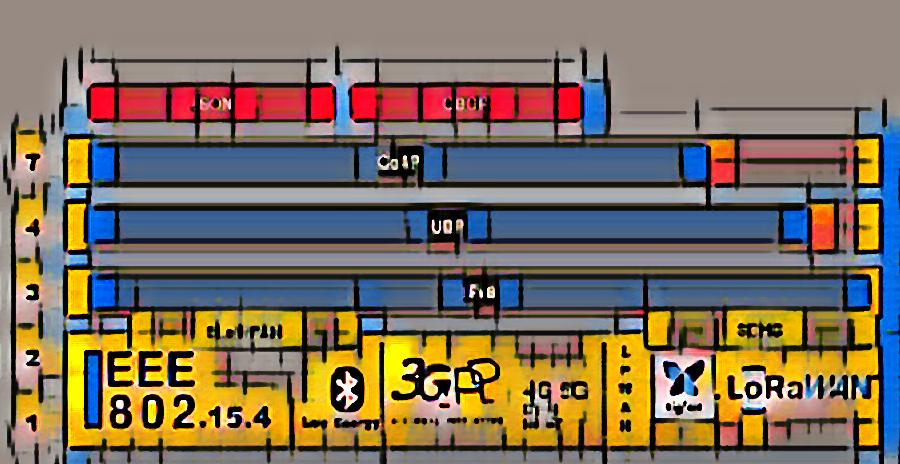
\includegraphics[scale=.70]{Pictures/cover.jpeg}}} % Image background
\centering
\vspace*{5cm}
\par\normalfont\fontsize{35}{35}\sffamily\selectfont
\lgf{\textbf{PROGRAMMER L'INTERNET DES OBJETS }}
\lge{\textbf{PROGRAMMING THE INTERNET OF THINGS }}
{\LARGE }\par % Book title
\vspace*{1cm}
{\Huge Laurent TOUTAIN}\par % Author name
\endgroup

%----------------------------------------------------------------------------------------
%	COPYRIGHT PAGE
%----------------------------------------------------------------------------------------

\newpage
~\vfill
\thispagestyle{empty}

%\noindent Copyright \copyright\ 2014 Andrea Hidalgo\\ % Copyright notice

\noindent \textsc{IMT Atlantique}\\
\doclicenseThis

\noindent \lgf{Basé sur le \href{https://bit.ly/3Ku0aL8}{MOOC PLIDO}.}\\ % License information
\lge{Based on the  \href{https://bit.ly/3Ku0aL8}{PLIDO MOOC}.} \\
\noindent \textit{\lgf{Publié le \today}\lge{Published \today}} % Printing/edition date

%----------------------------------------------------------------------------------------
%	TABLE OF CONTENTS
%----------------------------------------------------------------------------------------


\chapterimage{pano-tv1.png} % Chapter heading image

\pagestyle{empty} % No headers

\ifthenelse{\boolean{lfrench}}{
\renewcommand\contentsname{Table des Matières}
\renewcommand{\bibname}{Bibliographie}
}{}
\ifthenelse{\boolean{lenglish}}{
\renewcommand\contentsname{Table of Contents}
\renewcommand{\bibname}{Bibliography}
}{}

\cleardoublepage
\tableofcontents% Print the table of contents itself

%\cleardoublepage % Forces the first chapter to start on an odd page so it's on the right

\pagestyle{fancy} % Print headers again

%----------------------------------------------------------------------------------------
%	CHAPTERS
%----------------------------------------------------------------------------------------
\cleardoublepage

\lgf{\chapter*{Acronymes}}
\lge{\chapter*{Acronyms}}

\begin{multicols}{2}
\begin{acronym}
\acro{3GPP}{3rd Generation Partnership Project}
\acro{ABP}{Authentication By Personalisation}
\acro{ADSL}{Asymmetric Digital Subscriber Line}
\acro{AMQP}{Advanced Message Queuing Protocol}
\acro{AS}{Application Server}
\acro{ASCII}{American Standard Code for Information Interchange}
\acro{BLE}{Bluetooth Low Energy}
\acro{CBOR}{Concise Binaire Object Representation}
\acro{CoAP}{Constrained Application Protocol}
\acro{Cosem}{Companion Specification for Energy Management}
\acro{CRC}{Cyclic Redundancy Check}
\acro{CSV}{Comma Separated Values}
\acro{DLMS}{Device Language Message Specification}
\acro{DTT}{Digital Terrestrial Television}
\acro{DR}{Data Rate}
\acro{GSMA}{GSM Association}
\acro{HTML}{HyperText Markup Language}
\acro{HTTP}{HyperText Transport Protocol}
\acro{HTTPS}{HyperText Transport Protocol Secure}
\acro{IANA}{Internet Assigned Numbers Authority}
\acro{IBAN}{International Bank Account Number}
\acro{IEEE}{Institute of Electrical and Electronics Engineers}
\acro{IETF}{Internet Engineering Task Force}
\acro{IoT}{Internet of Things}
\acro{IP}{Internet Protocol}
\acro{IPv4}{Internet Protocol version 4}
\acro{IPv6}{Internet Protocol version 6}
\acro{IPSO}{IP for Smart Objects}
\acro{ITU}{International Telecommunication Union}
\acro{IRI}{International Resource Identifier}
\acro{ISBN}{International Standard Book Number}
\acro{ISO}{International Standardization Organization}
\acro{JMS}{Java Messaging Service}
\acro{JSON}{JavaScript Object Notation}
\acro{JSON-LD}{JavaScript Object Notation  for Linked Data}
\acro{LCIM}{Levels of Conceptual Interoperability Model}
\acro{LPWAN}{Low Power Wide Area Network}
\acro{LwM2M}{Lightweight Machine to Machine}
\acro{LNS}{LoRaWAN Network Server}
\acro{MQTT}{Message Queuing Telemetry Transport}
\acro{NAT}{Network Address Translation}
\acro{NGW}{Network GateWay}
\acro{NIDD}{Non IP Data Delivery}
\acro{OMA}{Open Mobile Alliance}
\acro{OTAA}{Over The Air Authentication}
\acro{OVH}{On Vous Herbèrge}
\acro{PAC}{Porting Authorization Code}
\acro{REST}{REpresentational State Transfer}
\acro{RFC}{Request For Comments}
\acro{RGW}{Radio GateWay}
\acro{RNIPP}{Répertoire National d'Identification des Personnes Physiques}
\acro{RSSI}{Received Signal Strength Indicator}
\acro{RTT}{Round Trip Time}
\acro{SCEF}{Service Capability Exposure Function}
\acro{SenML}{Sensor Measuring List}
\acro{SCHC}{Static Context Header Compression}
\acro{SF}{Spreading Factor}
\acro{SNR}{Signal to Noise Ratio}
\acro{SSID}{Service Set IDentifier}
\acro{STIC}{Sciences et Technologies de l’Information et de la Communication}
\acro{TCP}{Transmission Control Protocol}
\acro{TLV}{Type Length Value}
\acro{TNT}{Télévision Numérique Terrestre}
\acro{TTN}{The Things Network}
\acro{UDP}{User Datagram Protocol}
\acro{UIT}{Union internationale des télécommunications}
\acro{UNB}{Ultra Narrow-Band}
\acro{URI}{Universal Resource Identifier}
\acro{URL}{Univeral Resource Locator}
\acro{URN}{Univeral Resource Name}
\acro{VPS}{Virtual Private Server}
\acro{W3C}{World Wide Web Consortium}
\acro{WWW}{World Wide Web}
\acro{XML}{Extensible Markup Language}
\acro{XMPP}{Extensible Messaging Protocol et Presence}
\end{acronym}
\end{multicols}

\setboolean{allchap}{true} % true: take all, false take nothing only /input



\Input{Part00-liminaire}
\Input{Part01.0-Intro}
\Input{Part02.0-ArchiIP}
\Input{Part02.5-Wireshark}
\Input{Part03.0-Modbus}
\Input{Part04.0-ArchiIoT}
\Input{Part05.0-Data}
\Input{Part06.0-VSensors}
\Input{Part06.5-beebotte}
\Input{Part07.0-LoPy}
\Input{Part08.0-Sigfox}
\chapter{LoRaWAN}


\begin{wrapfigure}{r}{4cm}

\includegraphics[width=.3\columnwidth]{Pictures/LORAWAN-logo.png}
\end{wrapfigure}


Avec \Index{Sigfox}, ce n’était que du bonheur ! Nous avions un environnement unique développé par un seul acteur. L’attachement d’un objet au réseau, la récupération des données s’en trouve grandement simplifiée.

Avec \Index{LoRaWAN}, l'écosystème est plus complexe. Pour rappel, \Index{LoRa} est une modulation longue portée et LoRaWAN un protocole de niveau 2 qui a pour but de fédérer les acteurs (fabricants d’objets, utilisateurs d’objets, opérateur de réseaux) autour de la communication radio entre l’objet et le cœur de réseau appelé ici \ac{LNS} . Mais l’enregistrement des objets, le lien entre les applications et le LNS diffèrent d’un réseau à un autre.

     \vspace{1em}

Même si vous n’avez pas l’intention de mettre en œuvre le réseau Sigfox, nous vous recommandons de lire le chapitre précédent (ou à la rigueur de le survoler) car nous y ferons référence dans la suite du texte.

     \vspace{1em}

LoRaWAN, comme Sigfox, opère dans la même bande de fréquences non licenciées. Il existe plusieurs opérateurs de réseaux LoRaWAN :

\begin{itemize}
    \item  \ac{TTN}\footnote{\url{https://www.thethingsnetwork.org/}} propose une approche communautaire. Chaque personne peut mettre à disposition des passerelles radio pour la communauté et inscrire des objets. TTN gère le cœur de réseau. Si cette approche est sympathique, la couverture va être très parcellaire et va dépendre de la densité de geeks dans une région. De plus, la couverture du réseau va dépendre de la position des antennes qui doivent être placées sur un point haut. Avoir une antenne sur son balcon n’implique pas une grande couverture de la zone. Si vous avez de la chance, vous pourrez peut-être bénéficier d’un accès via TTN. Nous verrons comment s’y connecter.
    \item des opérateurs nationaux comme, en France, \Index{Orange} ou \Index{Bouygues Télécom}. Mais il faut généralement bourse délier pour connecter les objets et pour limiter l’usage du downlink ; l’envoi des messages vers les capteurs est facturé en supplément. En revanche, la couverture est supérieure.
    \item les réseaux privés. Il est possible de faire tourner son propre LNS. Cela implique d’acheter des composants pour faire une passerelle radio. Mais il existe des mises en oeuvre ouvrete du LNS comme \Index{chirpstack}\footnote{\url{https://www.chirpstack.io/}}. 

\end{itemize}

\section{Information sur le LoPy}

Chaque objet va avoir un identifiant unique codé sur 64 bits appelé \textit{\Index{devEUI}}. Cette information est nécessaire pour faire entrer un équipement sur le réseau. Le programme \lprog{lorawan\_devEUI.py}{pycom} donne accès à cette valeur qui est unique pour chaque LoPy.

\pycomlst{lorawan\_devEUI.py}\label{prog-devEUI}

L’objet Python \pfunction{network}{LoRa} est importé du module \texttt{network} et une instance est créée ligne 5. La variable \texttt{mac} va stocker l’adresse MAC (autre nom du \textit{devEUI}) retournée par l’objet \texttt{lora} et l'afficher en hexadécimal, comme le montre l’exemple suivant~:

\begin{termc}[backgroundcolor=\color{gray!10}, basicstyle=\ttfamily\small, escapechar=@] 
>>> Running lorawan_devEUI.py

>>>
>>>
devEUI:  b'70b3d54994c61237'
\end{termc}

On a le \textit{devEUI}. Il manque encore 3 informations :

\begin{itemize}
    \item \textit{\Index{appEUI}} : c’est un identifiant sur 64 bits comme le \textit{devEUI} qui va servir à identifier l’application. On peut le mettre à 0 ;
   \item \textit{\Index{AppKey}} : c’est une valeur sur 128 bits qui n’est connue que de l’objet et du LNS. Elle permet de dériver les clés de chiffrement utilisées par la suite ;

\end{itemize}

     \vspace{1em}

Et sur le LNS, il faudra aussi configurer le connecteur~: il s’agit d’indiquer au LNS comment envoyer les données vers une application. Il peut s’agir de POST HTTP comme nous avons vu avec la configuration du \textit{\Index{backend}} avec Sigfox. Bien entendu, une fois ces grands principes établis, ça serait trop simple si tous les réseaux fonctionnaient de la même façon. Nous allons donc voir comment faire avec le réseau TTN. 

\section{The Things Network}


\begin{wrapfigure}{r}{3cm}
\Youtube{https://youtu.be/G69mjg80-mA}
\end{wrapfigure}


The Things Network, ou TTN pour les intimes, est un réseau communautaire qui permet à tout un chacun de connecter soit une passerelle radio pour le bénéfice de la communauté, soit un objet. TTN se charge de faire tourner un LNS et de renvoyer les informations collectées à son propriétaire .On espère qu'un bon samaritain a déployé une antenne près de chez vous pour capter votre trafic. On n'a aucun moyen de savoir, si on n'essaye pas. 

     \vspace{1em}

La première étape consiste à se créer un compte, gratuit comme il se doit, sur le site de TTN~: \url{https://www.thethingsnetwork.org/}.

     \vspace{1em}


Une fois le formulaire de création de compte rempli et validé, vous disposez d’un accès au réseau TTN. 
Votre identifiant apparaît en haut à droite de la page Web. 

\begin{itemize}
    \item Cliquez sur votre nom,
    \item sélectionnez Console,
    \item puis votre zone géographique (cela n'a rien à voir avec le plan de fréquence. Il est préférable de choisir le serveur le plus proche pour optimiser les communications).
\end{itemize}


On peut soit définir une application et y associer des objets, soit connecter une passerelle radio (\textit{Go To Gateways}). Par la suite, nous explorerons cette option si vous voulez installer votre propre passerelle radio. Nous allons nous intéresser à la création d'application en choisissant \textit{Go To Applications}. TTN vous invite à créer notre première application ; cliquez sur le lien \textit{+Add Application}.

\subsection*{Définir une application}

Une application pour TTN va intégrer plusieurs objets LoRaWAN qui enverrons leur information à une application tournant sur un \ac{AS}. 
Il faut remplir le formulaire (cf. figure~\vref{fig-ttn-app}) en indiquant :
\begin{itemize}
    \item l'identifiant de l'application. Il s'agit d'un nom uniquement composé de lettres et de chiffres ainsi que du tiret. Il doit être unique pour TTN. Donc, faites preuve d'imagination car il doit être unique pour TTN. Ce nom se retrouvera dans les URI permettant de piloter l'application ;
    \item le nom de l'application qui apparaîtra dans les menus. Il n'y a pas de contraintes ; il vaut mieux choisir quelque chose d'explicite ;
    \item une description de l'application si nécessaire.
\end{itemize}

\begin{figure}[tbp]
\centerline{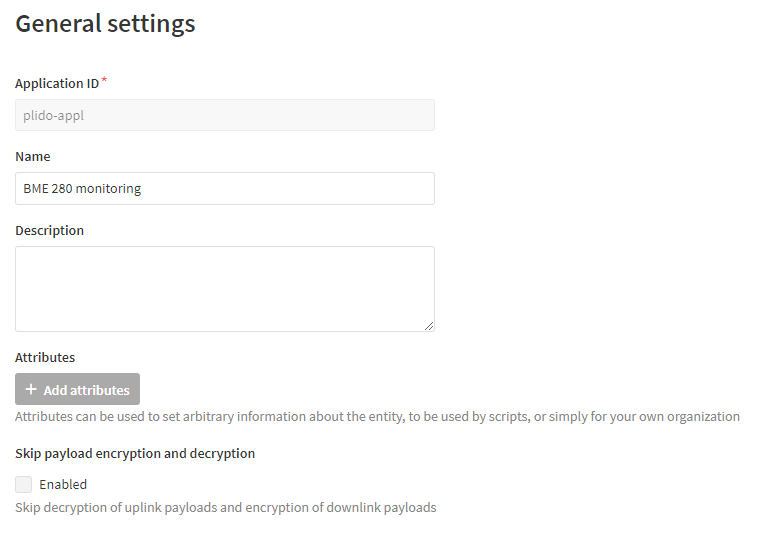
\includegraphics[width=0.7\columnwidth]{Pictures/ttn-app.png} }
\caption{Configuration d'une application.}
\label{fig-ttn-app}
\end{figure}

     \vspace{1em}

Cliquez sur Create Application pour enregistrer cette application. Vous arrivez sur un page de contrôle de votre application.

\subsubsection*{Ajout d'un objet}

Nous devons enregistrer un ou plusieurs objets dans notre application~:

\begin{itemize}
    \item Cliquez sur \textit{end devices} dans le menu de gauche~;
    \item puis \textit{+ Add end device}~;
    \item et \textit{try manual registration} en dessous du menu déroulant. TTN offre des aides à la configuration pour certains objets, mais comme nous sommes des experts, nous n'en n'avons pas besoin.
\end{itemize}

     \vspace{1em}


Le menu, décrit figure~\vref{fig-ttn-device} apparaît~:

\begin{figure}[tbp]
\centerline{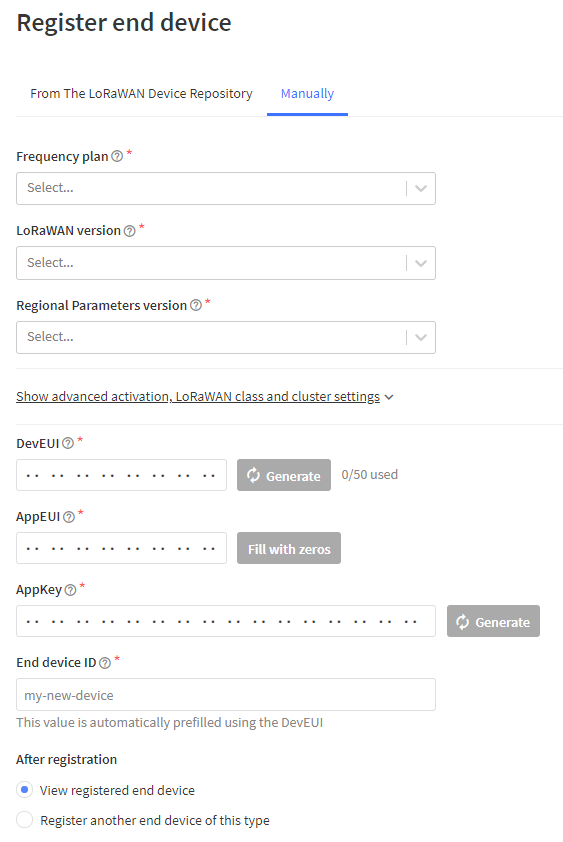
\includegraphics[width=.7\columnwidth]{Pictures/ttn-device.png} }
\caption{Ajout d'un objet.}
\label{fig-ttn-device}
\end{figure}

\begin{itemize}
    \item Entrez le plan fréquence compatible avec votre région. En Europe, vous pouvez choisir d'avoir la voie descendante en SF9~\footnote{Le \acl{SF} definit la vitesse de transmission de l'information, elle diminue de moitié à chaque incrémentation doc le SF12 est 16 fois plus lent que le SF9, mais beaucoup plus robuste.} ou en SF12. Le premier est un bon compromis entre la portée et la durée d'émission ; le second est à choisir si votre objet est difficilement accessible (profondément enfoui ou loin d'une passerelle radio) ;
    \item la version du protocole LoRaWAN compatible avec les LoPy  :\texttt{MAC V1.0.2}~;
    \item les paramètres de la couche physique du LoPy : \texttt{PHY V1.0.2 REV A}~;
    \item Vous devez récupérer le \textit{devEUI} de votre LoPY en lançant sur Atom le programme \lprog{lorawan\_devEUI.py}{pycom} (cf. Listing~\vref{prog-devEUI})~;
    \item mettez l'\textit{\Index{AppEUI}} à 0,
    \item et générez une clé de chiffrement \textit{\Index{AppKey}} et n'oubliez surtout pas de copier sa valeur quelque part, on en aura besoin pour configurer notre objet.
    
         \vspace{1em}

L'interface de TTN vous propose un identifiant pour l'objet basé sur son \textit{devEUI}. Vous pouvez le garder, à moins de vouloir quelque chose de plus explicite.

         \vspace{1em}

Finalement, cliquez sur \textit{register end device} pour sauvegarder votre oeuvre.

         \vspace{1em}

L'interface affiche une page récapitulative. Si vous avez oublié de le faire à l'étape précédente, copiez l'\textit{AppKey} pour la mettre dans le programme \lprog{lorawan\_send\_and\_receive.py}{pycom}.
\end{itemize}

\subsubsection*{Connexion de l'objet}

\pycomlst[firstline=1,lastline=10, firstnumber=1]{lorawan\_send\_and\_receive.py}

Le programme \lprog{lorawan\_send\_and\_receive.py}{pycom} commence, comme \lprog{lorawan\_devEUI.py}{pycom}, par créer un objet \texttt{lora} et afficher le \textit{devEUI} de l'objet, c'est toujours partique pour le deboguage.


\pycomnxt[firstline=12,lastline=18, firstnumber=12]{lorawan\_send\_and\_receive.py}

On met dans deux variables, les identifiants présents sur le LNS de TTN, à savoir le \textit{app\_eui} que l'on avait mis à zéro et de \textit{app\_key} que l'on généré aléatoirement sur le site de TTN et que l'on vous avait demandé de copier quelque part.

Pour éviter de manipuler des séquences binaires, ces valeurs sont vues comme des chaînes de caractères (des espaces peuvent être insérés pour plus de lisibilité, la fonction \texttt{replace} permet de les éliminer). La séquence binaire est obtenue grâce à la fonction \pfunction{binascii}{unhexlify}.


\pycomnxt[firstline=19,lastline=20, firstnumber=19]{lorawan\_send\_and\_receive.py}

On arrête le clignotement périodique bleu de la LED du LoPy en appelant la pfunction{pycom}{heartbeat} avec l'argument \texttt{False}. Puis on allume la LED en blanc avec la fonction \pfunction{pycom}{rgbled}. L'argument donne l'intensité des trois composantes Rouge, Vert et Bleu. 

La LED va nous permettre de suivre pas à pas l'état du LoPy.

\pycomnxt[firstline=22,lastline=30, firstnumber=22]{lorawan\_send\_and\_receive.py}

Le LoPy effectue la connexion au réseau, cette procédure est appelée \textit{\Index{Join}}. Elle correspond à l'émission d'un message vers le LNS. Si celui-ci reconnaît et accepte l'objet, il renverra quelques secondes plus tard un message \texttt{Accept}. Cette phase permet à l'Objet d'obtenir les clés de chiffrement des messages et une adresse plus courte appelé \textit{\Index{devAddr}}.

Pour se faire, le programme appelle la fonction \pfunction{lora}{join} avec les paramètres suivants~: 
\begin{itemize}
    \item e type de connexion, très souvent \ac{OTAA} pour récupérer dynamiquement les paramètres\footnote{Il existe aussi une méthode appelé \ac{ABP} qui consiste à configurer l'objet avec tous ses paramètres (comme pour Sigfox), mais elle est moins souple et moins adaptée à l'environnement LoRaWAN où plusieurs opérateurs coexistent sur les mêmes fréquences.}  
    \item les paramètres nécessaires, à savoir l'\textit{AppEUI} et l'\textit{AppKey} que nous avons précédemment configurés.
    \item un temporisateur (\textit{timeout}). La valeur à 0 indique que l'objet va essayer de joindre le réseau jusqu'à ce que celui-ci l'accepte.
\end{itemize}
         \vspace{1em}

La fonction \pfunction{lora}{join} n'étant pas bloquante, la procédure de \textit{join} va se dérouler en tâche de fond. La fonction \pfunction{lora}{has\_joined} permet de suivre l'état du LoPy. D'où la boucle (lignes 26 à 28) dont on ne sortira que lorsque le LoPy sera accepter sur le réseau. 

Toutes de 2.5 seconde un message sera affiché pour dire qu'il est toujours en attente d'une réponse. Ces messages ne sont absolument pas synchronisés avec l'envoi des trames \texttt{Join} qui ont lieu toutes les 15 secondes.

L'extinction de la LED (ligne 30) indique que le LoPy a joint le réseau LoRaWAN.

\pycomnxt[firstline=32,lastline=34, firstnumber=32]{lorawan\_send\_and\_receive.py}

Le programme ouvre la socket, le premier paramètre est \texttt{\Index{AF\_LORA}} pour indiquer que l'on utilise le protocole LoRaWAN. Les deux lignes suivantes, avec les fonctions \pfunction{socket}{setsockopt}, permettent de configurer des paramètres LoRaWAN, comme~:
\begin{itemize}
\item le \ac{DR}. Sous ce terme, plusieurs paramètres des la couche physique sont réunis. Plus le \ac{DR} est élevé, plus la transmission est rapide. En contre partie, elle est moins robuste et peut porter moins lion. Le \ac{DR} varie entre 0 et 6.
\item la capacité de LoRaWAN a acquitter les trames. Il n'est pas recommandé de l'activer car cela induit des émissions qui sont prises en compte dans le calcul du \Index{Duty Cycle} (voir chapitre~\vref{chap-star}).
\end{itemize}



\pycomnxt[firstline=36,lastline=46, firstnumber=36]{lorawan\_send\_and\_receive.py}

On entre dans une boucle sans fin pour envoyer et recevoir périodiquement des messages~:
\begin{itemize}
    \item ligne 37, la LED éclaire en rouge pour indiquer une transmission.
    \item ligne 38, les appels aux sockets sont rendu bloquant, c'est-à-dire qu'il ne finiront que quand l'action sera effectuée par la couche inférieure.
    \item ligne 39, par contre au bout de 10 secondes d'attente une erreur sera déclanchée.
    \item ligne 41, on récupère cette erreur grâce aux instructions \texttt{\Index{try}} et \texttt{\Index{except}} de Python. Si l'appel à \pfunction{socket}{send} reste bloqué plus des 10 secondes, le traitement de l'exception affiche \texttt{timeout in sending}. Cet événement est rare et est causé par une défaillance locale à la couche 2\footnote{Il faut rester vigilant sur cette erreur, par exemple si l'on essaie d'envoyer un entier sans sérialisation, cela conduira à une erreur qui sera prise en compte de cette manière.}.
    \item ligne 46 dans tous les cas, la LED passe en bleu.
\end{itemize}

\pycomnxt[firstline=49,lastline=59, firstnumber=49]{lorawan\_send\_and\_receive.py}

Finalement, on attend des données. Dans le mode le plus fréquent de LoRaWAN, un équipement ne peut recevoir des données que dans une courte fenêtre après une émission. Si des données arrivent en dehors de cette fenêtre, le LNS mémorise l'information et la transmettra quand il recevra une trame de l'objet. Cela permet d'économiser beaucoup d'énergie car le capteur peut dormir de ses deux oreilles, il sait qu'il ne manquera pas une information.

La voie descendante est une ressource rare, et il ne faut généralement pas trop l'utiliser\footnote{TTN ne facture pas les données descendantes, mais d'autres opérateurs le font, faites attention si vous adaptez ces exemples à d'autres environnements, car dans les premiers tests, nous utiliseront la voie de retour.}, donc il ne devrait pas y avoir souvent de messages en retour. Sauf ici, pour tester toute la chaîne de transmission~:
\begin{itemize}
    \item ligne 49, l'appel à \pfunction{socket}{recv} est aussi bloquant tant que des données ne sont pas arrivées. 
    \item lignes 51 et 52, si des données arrivent, elles sont affichées et la LED passe au vert.
    \item lignes 53 à 55, si aucune données arrivent, le temporisateur se déclenche au bout de 10 secondes générant l''exception. Un message averti l'utilisateur de l'absence de données et la LED est éteinte.
\end{itemize}

         \vspace{1em}

Si tout va bien, qu'une passerelle radio est à portée de votre objet, le programme  \lprog{lorawan\_send\_and\_receive.py}{pycom} va se connecter au réseau après avoir affiché 3 fois \texttt{Not yet joined...}~:


\begin{termc}[backgroundcolor=\color{gray!10}, basicstyle=\ttfamily\small, escapechar=@] 
>>> Running lorawan_send_and_receive.py

>>>
>>>
devEUI:  b'70b3d54994c61237'
Not yet joined...
Not yet joined...
Not yet joined...
timeout in receive
timeout in receive
\end{termc}


\noindent correspondant au 5 secondes prévues par le standard avant d'envoyer le message d'acceptation de l'objet. 
La LED passe du blanc au rouge indiquant qu'un message a été émis puis doit s'éteindre et le message \texttt{timeout in receive} est affiché indiquant que l'Objet n'a pas reçu de message en réponse à son émission.

\subsubsection{Analyse des traces}

Côté LNS, il est possible de voir le trafic sur la page résumant les caractéristiques de l'objet dans la fenêtre \textit{live data} (cf. figure~\vref{fig-lora-join}).

\begin{figure}[tbp]
\centerline{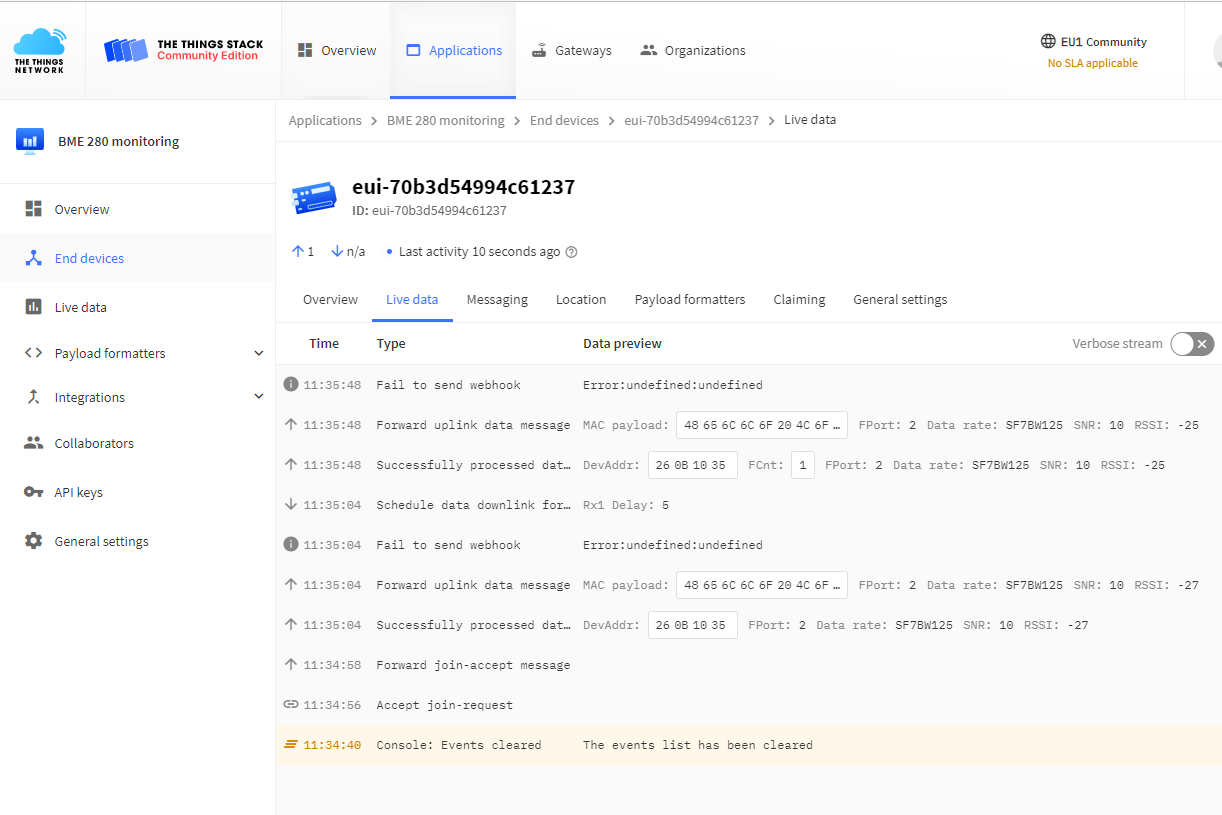
\includegraphics[width=.7\columnwidth]{Pictures/lora-join.png} }
\caption{Trace d'un objet.}
\label{fig-lora-join}
\end{figure}

Les événements sur la figure se lisent de bas en haut comme le confirme l'horodatage, en cliquant sur la ligne correspondante, TTN affiche les messages JSON utilisés par le LNS pour traiter l'information. On y retrouve les données échangées~:

\begin{itemize}
    \item L'événement \textit{Accept \Index{Join-request}} indique que le LNS a reçu le message Join de l'objet, indiquant qu'il voulait rejoindre le réseau. Le LNS l'a traité, a vérifié qu'il y avait un objet déclaré avec le bon \textit{\Index{devEUI}} et que l'\textit{\Index{AppKey}} utilisée par l'objet pour signer sa demande était identique à la valeur configurée. Dans la trace suivante, on peut retrouver le \textit{\Index{devEUI}} de l'objet et la \textit{\Index{devAddr}}, qui lui a été attribuée temporairement. Cette dernière sera utilisée par la suite.
    
\begin{termc}[backgroundcolor=\color{blue!10}, basicstyle=\ttfamily\small, escapechar=@] 
    "device_ids": {
        "device_id": "eui-70b3d54994c61237",
        "application_ids": {
          "application_id": "plido-appl"
        },
        "dev_eui": "70B3D54994C61237",
        "join_eui": "0000000000000000",
        "dev_addr": "260B1035"
      }
\end{termc}

    \item L'événement \textit{Forward \Index{Join-accept} message} indique que le LNS envoie un message d'acceptation à l'Objet. Ce message est différé de 5 secondes pendant lesquelles l'Objet dort. 
    
    \item L'événement \textit{Successfully processed data message} montre que le LNS a reçu correctement le message de données émis par l'Objet. La trace donne des indications sur certains paramètres physique, tels que le \acl{SF} (ici SF7 soit la modulation la plus rapide et la moins robuste), le SNR qui indique le ratio entre la puissance du signal reçu par rapport au bruit et le \ac{RSSI} donnant la force du signal.   
    
    
    \item L'événement \textit{Forward uplink data message} donne plus d'information sur le message et son contenu. Le champs \texttt{frm\_payload} donne le contenu déchiffré par le LNS mais codé en \Index{base64}. On y retrouve le message d'origine \texttt{Hello LoRa}. 
\begin{termc}[backgroundcolor=\color{blue!10}, basicstyle=\ttfamily\small, escapechar=@] 
    "uplink_message": {
      "session_key_id": "AX4VNOuMbClcPKF63sKy6A==",
      "f_port": 2,
      "frm_payload": "SGVsbG8gTG9SYQ==",
      "rx_metadata": [
        {
          "gateway_ids": {
            "gateway_id": "gateway-lo",
            "eui": "B827EBFFFE08F8A8"
          },
          "time": "2022-01-01T10:35:04.247807Z",
          "timestamp": 2661650827,
          "rssi": -27,
          "channel_rssi": -27,
          "snr": 10,
          "uplink_token": "ChgKFgoKZ2F0ZX....",
          "channel_index": 1
        }
      }
\end{termc}


\end{itemize}


    
\Question{Mauvais appKey}
{Quel message de trace obtenez vous du LNS, si l'Objet n'est pas configuré avec le même \yexyit{\Index{AppKey}} que le LNS~?}
{
\texttt{12:52:11 Join-request to cluster-local Join Server failed MIC mismatch}\\
\texttt{12:52:01 Join-request to cluster-local Join Server failed MIC mismatch}\\
\texttt{12:51:51 Join-request to cluster-local Join Server failed MIC mismatch}\\

}

\Question{Autonomie}
{Quel impact sur les batteries~?}
{Le LoPy va émettre périodiquement tous les 10 secondes un message de type \Index{Join-request}. Le but est pouvoir se connecter, même si la transmission n'est pas optimale. mais en cas de mauvaise configuration, cela va se traduire par une occupation plus importante du réseau, mais surtout un impact sur l'autonomie de l'Objet.}

Le \Index{fPort} que l'on retrouve dans les trames de données LoraWAN permet d'indiquer le programme qui va traiter l'information. La valeur 0 est spéciale et indique une trame de configuration de la couche LoRaWAN, les autres valeurs jusquà 223 désignent des applications spécifiques. Bien qu'il soit peu utilisé, il est parfois utile de la changer. 

\Question{fPort}
{Dans les traces précédentes, quelle est la valeur du fPort par défaut utilisé par le LoPy~? }
{\texttt{  "f\_port": 2,}}

\Question{Changement de fPort}
{L'instruction \pfunction{socket}{bind} permet de modifier le \Index{fPort} pour une transmission. Modifiez le programme pour utiliser le fPort 10 et vérifiez l'effet dans les traces de TTN. }
{Le programme doit être modifié par exemple après les instructions \pfunction{socket}{setsockopt} en ajoutant la ligne~:\\
\texttt{s.bind(10)}\\
}

\subsubsection{Configuration du connecteur}

Le LNS n'a pas été configuré pour envoyer le message à un Serveur d'Application (\acl{AS}). Comme pour \Index{Sigfox}, il faut définir une URI pour indiquer au LNS où poster les données.

         \vspace{1em}


Pour configurer un connecteur, il faut aller sur le menu de gauche \textit{Integrations}. TTN propose des intégrations directes avec des services cloud existants, mais il est également possible de configurer son propre connecteur~:
\begin{itemize}
    \item via \Index{MQTT}, TTN joue le rôle de \Index{\textit{broker}} et fourni le nom du \Index{topic} et le secret.
    \item en stockant localement des données par le choix \textit{\Index{Storage integration}} et en y accédant par une requête GET, comme Sigfox le propose (cf. chapitre~\vref{chap-sigfox-GET}). Cela permet de recevoir les données si l'on est situé derrière un \ac{NAT}, mais rend la réception asynchrone puisque l'application doit interroger régulièrement le serveur de TTN.
    \item en configuration une URI sur le serveur pour que celui-ci produit une requête POST quand une trame de donnée est reçue (choix \textit{\Index{Webhooks}}).
\end{itemize}

         \vspace{1em}

Nous allons également privilégier pour TTN ce dernier mode de fonctionnement, car si il nécessite une configuration du \ac{NAT}, il permet de recevoir les données de manière synchrone lorsqu'elles sont traitées par le LNS.


Il faut cliquer sur \Index{Webhooks}. Un certain nombre de services sont proposés, mais nous allons définir le nôtre à l'instar de ce que nous avons fait avec Sigfox (cf. chapitre~\vref{chap-sigfox-POST}). Pour préparer la connectivité, il est nécessaire~:
\begin{itemize}
    \item Si vous êtes dans le cloud, l'adresse s'obtient en tapant la commande \texttt{\Index{ifconfig}}.
    \item Si vous êtes derrière une box ou le routeur de votre fournisseur d'accès, vous avez une adresse privée. Un site web comme \url{myip.wtf} vous retournera l'adresse IPv4 publique. Vous devez ensuite configurer votre router d'accès pour qu'il envoie les paquets TCP ayant le numéro de port 9999 à votre ordinateur.
\end{itemize}

         \vspace{1em}


Cela va permette de former l'URI suivante~:
\begin{termc}[backgroundcolor=\color{blue!10}, basicstyle=\ttfamily\small, escapechar=@]
http://@\textit{aaa.bbb.ccc.ddd}@:9999/ttn
\end{termc}

\noindent où \textit{aaa.bbb.ccc.ddd} représente l'adresse IP publique de votre équipement. Comme cette adresse peut changer au cours du temps, il est préférable d'utiliser un service de DNS dynamique pour obtenir un nom de domaine plus stable sur la durée.

         \vspace{1em}

La page listant les \textit{\Index{Webhooks}} associés à l'application est vide. Il faut cliquer sur \textit{} pour en ajouter un nouveau, il convient de choisir \textit{Custom webhook}, les autres définissent les connecteurs vers des services de gestion des données (cf. figure~\vref{fig-ttn-webhook}).

\begin{figure}[tbp]
\centerline{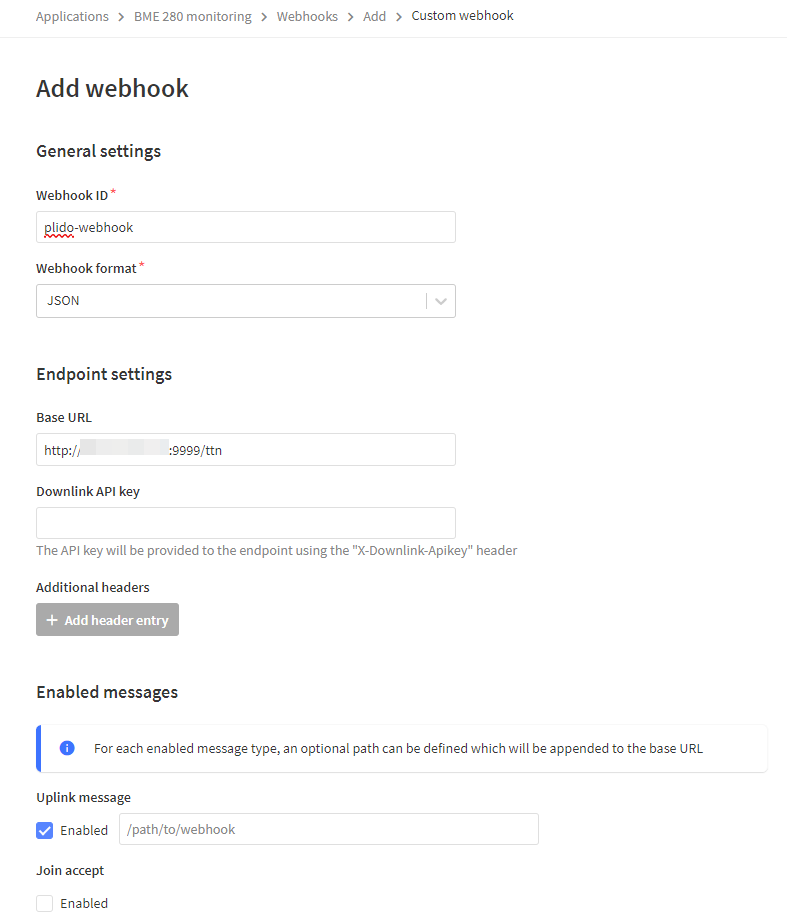
\includegraphics[width=.7\columnwidth]{Pictures/ttn-webhook.png} }
\caption{Configuration d'un webhook.}
\label{fig-ttn-webhook}
\end{figure}

Dans ce menu, il faut indiquer~:
\begin{itemize}
    \item l'identifiant du webhook~:
    \item le format JSON~:
    \item l'URI que nous venons de construire~:
    \item il n'est pas nécessaire pour l'instant de remplir la \textit{Download API Key} qui servira pour envoyer des données à l'Objet. Nous y reviendrons par la suite.
    \item il faut choisir les événements qui déclencheront une requête POST. Dans notre cas, on ne choisi que la récéption d'un message montant (\textit{Uplink message}).  On peut compléter le chemin de l'URI précédemment définie avec des éléments qui permettrons au serveur REST de mieux identifier le type de requête. Dans notre cas, cela n'est pas nécessaire. \texttt{/ttn} identifie par conséquent les messages reçus par le LNS des Objets.
\end{itemize}
Une fois le \textit{webhook} validé, le programme \pprog{generic\_relay.py}{plido-tp3} doit être lancé. Il va créer un serveur Web qui va attendre les requêtes POST du LNS de TTN.

         \vspace{1em}

 \pythonnxt[firstline=93,lastline=128, firstnumber=93   ]{generic\_relay.py}
 
 Ce programme utilise le module \Index{Flask} pour créer un serveur Web. Il associe le chemin \texttt{/ttn} à la fonction \texttt{get\_from\_ttn} pour les requêtes de type POST (lignes 93 et 94). Quand une requête de ce type arrive, la variable 
\texttt{fromGW} contient l'objet JSON\footnote{convertie implicitement en dictionnaire Python.} (ligne 95). Si elle contient la clé \texttt{uplink\_message}, les données sont extraites (ligne 100) pour être envoyé au travers de l'interface \textit{\Index{loopback}}  grâce à la fonction \texttt{\Index{forward\_data}} à un programme qui les traite. Si cette fonction retourne la valeur \texttt{None}, le programme ne souhaite pas répondre à l'Objet, le serveur Web acquitte positivement (code \texttt{200}) la requête venant du LNS (ligne 130 et 131).

\label{chap—forward-data}
 \pythonnxt[firstline=27,lastline=50, firstnumber=27]{generic\_relay.py}


Si le mode \texttt{verbose} est activé, le message à envoyer au programme de traitement des données est affiché en hexadécimal grâce à la fonction \pfunction{binascii}{hexlify} (lignes 33 et 34). Puis le message est effectivement émis (ligne 35)\footnote{l'adresse du destinataire et le port sont configurés lors de l'analyse des paramètres.}

Pour attendre une réponse qui n'est pas systématique, on ne peut pas utiliser l'appel \pfunction{socket}{recvfrom} car celui-ci est bloquant. A la place, on utilise l'appel \pfunction{select}{select} du module du même nom. Il permet d'attendre sur plusieurs événements à la fois provenant de différentes sockets (ligne 37) où~:
\begin{itemize}
    \item \texttt{inputs} est un tableau des sockets pouvant avoir reçu des données. Dans notre cas (ligne 30) il est initialisé avec la socket dialoguant avec le programme traitant les données~;
    \item \texttt{outputs} est un tableau qui contient les sockets dans lesquelles il serait possible d'écrire. Dans notre cas, ce tableau est vide (ligne 31).
    \item le troisième concerne les exceptions. Dans notre cas, on répète le tableau des sockets \texttt{inputs}
    \item finalement le quatrième praramètre indique la durée d'attente dans la fonction \pfunction{select}{select}. Dans notre cas, il est fixé à 0.1 seconde. ce temps est a la fois compatible avec une réponse du programme de traitement des données, et la réponse que l'on doit envoyer au LNS pour que la réponse soit associée au message montant.
\end{itemize}

\pfunction{select}{select} retourne dans un tuple de trois éléments, la ou les sockets qui ont déclenché son retour. Dans notre cas, se sont~:
\begin{itemize}
    \item soit l'expiration du temporisateur, dans ce cas, la variable \texttt{readable} qui contient la liste des sockets ayant recues des données est vide (ligne 39) et la valeur \texttt{None} est retournée.
    \item soit des données qui sont arrivées dans une ou plusieurs socket. la variable \texttt{readable} contient le tableau de ces sockets. La variable \texttt{s} contient la première socket du tableau, les données sont lues et envoyées en retour.
\end{itemize}


         \vspace{1em}

Le programme \pprog{generic\_relay.py}{plido-tp3}, lancé avec l'option \texttt{-v} montre de manière synthétique le trafic. 

\begin{termc}[backgroundcolor=\color{palerod}, basicstyle=\ttfamily\small, escapechar=@]
>python3 generic_relay.py -v
--UP-> b'48656c6c6f204c6f5261'
no DW
63.34.43.96 - - [01/Jan/2022 18:27:45] "POST /ttn HTTP/1.1" 200 -
--UP-> b'48656c6c6f204c6f5261'
no DW
34.255.49.188 - - [01/Jan/2022 18:28:31] "POST /ttn HTTP/1.1" 200 -
\end{termc}

Le contenu du message montant est affiché en hexadécimal et correspond au fameux contenu \texttt{Hello LoRa}. Comme il n'y a pas de réponse, \texttt{no DW} est ensuite affiché.

\subsubsection{Traitement des données}

La fonction \texttt{\Index{forward\_data}} du programme \pprog{generic\_relay.py}{plido-tp3} envoie les données à l'adresse de \textit{\Index{loopback}} \texttt{127.0.0.1} et sur le port \texttt{33033}\footnote{Ces deux valeurs peuvent être respectivement changées  en utilisant les arguments \texttt{-{}-forward\_address} et  \texttt{-{}-forward\_port}.}.

Le programmme \pprog{display\_receive\_and\_send.py}{plido-tp3} traite les données de l'Objet.

\pythonlst{display\_receive\_and\_send.py}

Il attend les données sur le port 33033. La fonction \pfunction{socket}{recvfom} retourne les données stockées dans la variable \texttt{data} et l'adresse de celui qui a envoyé les données stockée dans la variable \texttt{addr}. Les données sont affichée ligne 9 et le message \texttt{Pleased to meet you} est retourné à l'émetteur, en ligne 10 grâce à la fonction \pfunction{socket}{sendto}.

         \vspace{1em}

En lançant le programme dans une nouvelle fenêtre, on reçoit correctement le message du LoPy.

\begin{termc}[backgroundcolor=\color{palerod}, basicstyle=\ttfamily\small, escapechar=@]
>python3 display_receive_and_send.py
b'Hello LoRa'
\end{termc}

En revanche, le programme \pprog{generic\_relay.py}{plido-tp3} produit une erreur.

\begin{termc}[backgroundcolor=\color{palerod}, basicstyle=\ttfamily\small, escapechar=@]
--UP-> b'48656c6c6f204c6f5261'
<-DW-- b'506c656173656420746f206d65657420796f7521'
63.34.43.96 - - [01/Jan/2022 19:06:51] "POST /ttn HTTP/1.1" @\textcolor{red}{500}@ -
Traceback (most recent call last):
...
\end{termc}

Le message en retour a été reçu par la fonction \texttt{\Index{forward\_data}}, mais la voie descendante n'a pas encore été configurée. L'erreur est liée à l'absence du fichier \pprog{ttn\_config.py}{plido-tp3}, ligne 104, ce qui force Flask a retourner le status \texttt{500} et afficher les fonctions qui ont conduit à l'erreur.

\subsubsection{Voie retour}

Il n'y a aucun problème de sécurité quand le LNS envoie au serveur d'application des données reçues de capteurs, car l'endroit où il les transmet a été configuré par leur propriétaire. Par contre, dans l'autre sens, le LNS doit s'assurer que les données à transmettre à l'Objet, proviennent bien d'un serveur d'application autorisé.

Comme pour Beebotte, une clé secrète va être utilisée. A cette clé, le LNS peut associer des droits pour plus ou mois limiter les accès. Dans le menu de gauche, cliquez sur \textit{API key} puis sur \textit{+ Add API Key}. Dans l'écran suivant, donnez un nom à votre clé et choisissez \textit{Grant Individual Right} pour limiter l'usage de la clé. Sélectionnez \textit{Write downlink application traffic} et validez. 

         \vspace{1em}

Recopiez la clé et confirmer que vous l'avez bien fait en validant \textit{I have copied the key}. Editez le fichier \pprog{ttn\_config.py}{plido-tp3} en y insérant la clé obtenue.

\pythonlst{ttn\_config.py}

\begin{figure}[tbp]
\centerline{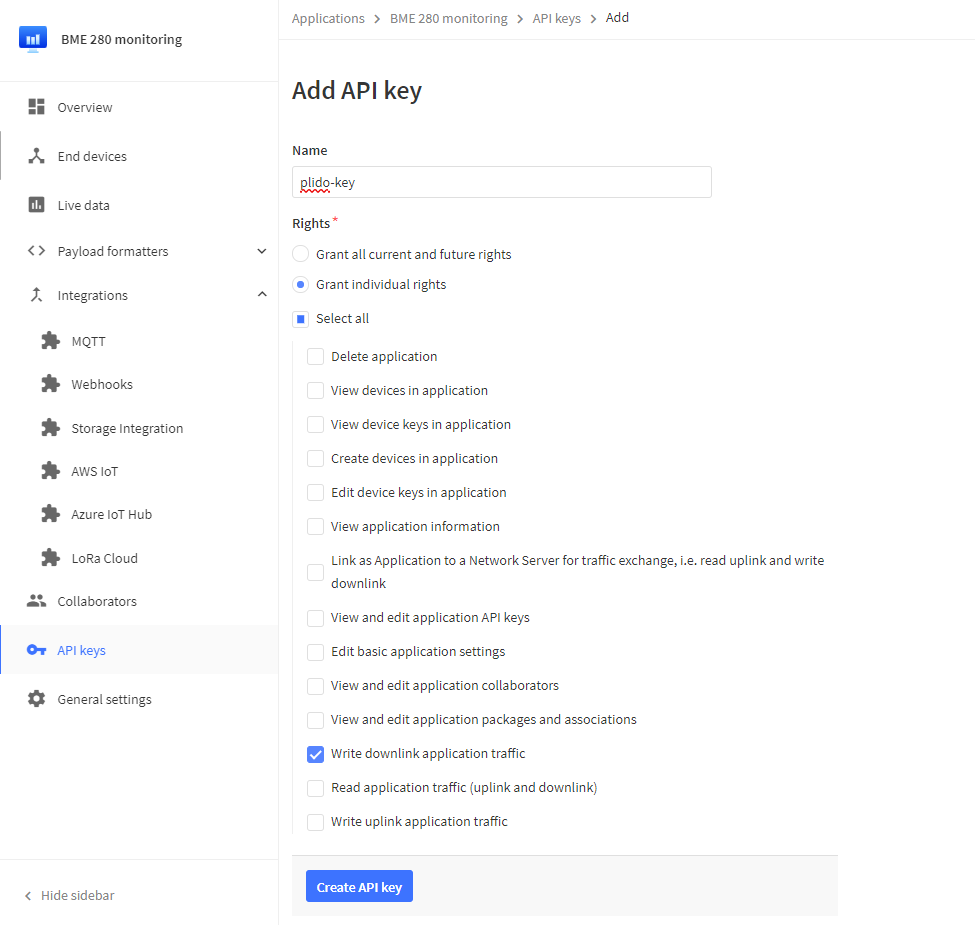
\includegraphics[width=.7\columnwidth]{Pictures/ttn-key.png} }
\caption{Création d'une clé}
\label{fig-ttn-key}
\end{figure}

Relancez le programmme \pprog{generic\_relay.py}{plido-tp3}, le LoPy  affiche la réponse.

         \vspace{1em}

Le listing suivant reprend la construction de la requête POST vers le LNS pour transporter le message descendant~:

 \pythonnxt[firstline=103,lastline=125, firstnumber=103]{generic\_relay.py}

\begin{itemize}
\item ligne 104, la clé autorisant l'envoi de message descendant est copié dans la variable \texttt{TTN\_Downlink\_Key}.
\item lignes 106 à 110, le format JSON attendu par le LNS pour envoyer un message descendant est construit, plusieurs messages peuvent être envoyés à la fois, d'où l'utilisation d'un tableau. Chacun des éléments contient un \texttt{\Index{fPort}} qui est recopié du message montant et des données qui proviennent de la socket (variable \texttt{downlink} codé en base64.

\begin{termc}[backgroundcolor=\color{palerod}, basicstyle=\ttfamily\tiny, escapechar=@]
{'downlinks': [{'frm_payload': 'UGxlYXNlZCB0byBtZWV0IHlvdSE=', 'f_port': 10}]}
\end{termc}
\item lignes 111 à 116, l'URI pour accéder au service est construite. Elle contient deux éléments variables qui identifient l'application et l'Objet. Ceux-ci sont également extrait du message montant.
\begin{termc}[backgroundcolor=\color{palerod}, basicstyle=\ttfamily\tiny, escapechar=@]
https://eu1.cloud.thethings.network/api/v3/as/applications/plido-appl/devices/eui-70b3d54994c61237/down/push
\end{termc}
\item lignes 118 à 121, les options qui seront ajoutées à l'en-tête HTTP sont indiquées. Elle contiennent la clé d'authentification.
\item finalement, ligne 123 à 125, ces différents élements sont passés à la fonction \pfunction{requests}{post} du module \texttt{requests}.
\end{itemize}



\section{Ajout d'une passerelle radio}

\begin{wrapfigure}{r}{3cm}
\Youtube{https://youtu.be/2VZRweC4fbo}
\end{wrapfigure}




Vous voulez installer une passerelle radio LoRaWAN chez vous pour bénéficier d'un réseau longue portée. Nous avons choisi d'utiliser un \Index{Pygate} qui nous permettra de rester dans l'univers Pycom que nous connaissons bien maintenant et surtout qui est une des solutions les moins chères. 

\subsection{Installation du Pygate}


Pour cela vous devez posséder un carte spécifique qui agit comme une carte d'extension. On y connecte un processeur. Ce dernier n'est pas forcément un LoPy car nous n'utiliserons pas sa partie radio LoRa. En effet, le Pygate dispose d'un autre composant radio Semtech qui permet l"écoute simultanée de huit canaux LoRa. Un LoPy lui ne peut écouter que sur un seul canal à la fois. En effet lors de l'émission d'une donnée, l'objet choisi aléatoirement un canal radio pour que le message soit reçu. Il faut que la passerelle radio écoute sur tous les canaux possibles.

         \vspace{1em}

\begin{wrapfigure}{r}{6cm}
\centerline{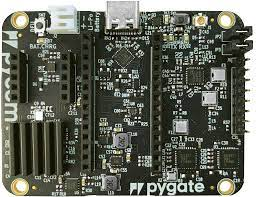
\includegraphics[width=.4\columnwidth]{Pictures/pygate.png}}
\end{wrapfigure}

On insère le Pycom sur la Pygate et on connecte l'antenne sur le connecteur du Pygate. Dans un second temps on doit adapter le Pycom à ses nouvelles fonctions, en téléchargeant le bon microprogramme. On le fait en lançant le programme Pycom Firmware Update et en choisissant Pygate. 

         \vspace{1em}


Dans un troisième temps, on ouvre le répertoire Pygate avec Atom. On y trouve le fichier \lprog{wifi\_conf.py}{Pygate} qui va permettre à la Gateway d'avoir accès à votre réseau wifi, il peut contenir les mêmes identifiants que lorsque vous aviez connecter votre LoPY à votre réseau wifi. Le programme \lprog{main.py}{Pygate} est préconfigurée pour utiliser le LNS européen de The Things Network. 

         \vspace{1em}

Le fichier \lprog{config.json}{Pygate} contient la description des fréquences utilisables dans cette zone. En y jetant un coup d'œil, on peut voir huit fréquences qui sont écoutées par la passerelle radio. Vous trouverez sur le site de The Things Network les autres configurations possibles. 

         \vspace{1em}


On téléverse le programme dans la mémoire du Pycom de la passerelle radio et comme il s'appelle \lprog{main.py}, il va se lancer tout seul au redémarrage. Il se connecte au wifi, puis va afficher l'identifiant la passerelle. Recopiez le car nous allons avoir besoin plus tard. Après on a plein de texte indiquant que la passerelle est en train de configurer le réseau LoRaWAN. Quand la led passe au vert, la passerelle est active. 

\subsection{Configuration de The Things Network}


Maintenant nous devons informer The Things Networks de l'existence de notre passerelle radio. Si ce n'est pas le cas vous devrez créer un compte sur The Things Network. Aller sur console choisissez \textit{Europe 1} si vous êtes en Europe ou la zone géographique correspondante. Ajoutez une passerelle en donnant : 
\begin{itemize}
    \item un identifiant textuel qui est un non lisible sans espaces~;
    \item l'identifiant de la passerelle qui correspond à la valeur hexadécimale affiché au démarrage~;
    \item un texte pour mieux décrire la passerelle~;
    \item finalement le plan fréquences\footnote{si les objets sont facilement accessibles on peut choisir le Spreading Factor 9 pour la voie descendante sinon si vous n'arrivez pas à joindre vos objets, vous pouvez vous replier sur le Spreading Factor 12}. 
\end{itemize}

On valide la passerelle et elle est ajoutée au LNS. Vous allez pouvoir visualiser les trames qu'elle reçoit.

\section{Vue générale des échanges}

La figure~\vref{fig-ttn-exchanges} en illustre le fonctionnement global. La première émission du LoPy est captée par un ou plusieurs passerelles radio, qui relaient le message via un format JSON spécifique appelé \textit{\Index{Packet Forwarder}}, cela peut être de directement en UDP ou en utilisant MQTT. Le LNS après identification de l'Objet, envoie une requête POST contenant les données émise vers une destination configurée par une URI. Cette requête arrive au routeur du domicile, qui l'envoie à un équipement dans le domicile en fonction de la configuration du NAT. 
Le programme \pprog{generic\_relay.py}{plido-tp3} traite la requête, en extrait le contenu et l'envoie via une socket au programme.
Si ce dernier ne répond pas, le temporisateur se déclenche et la requête est acquitée.

Sinon, si le  programme \pprog{generic\_relay.py}{plido-tp3} reçoit des données en réponse avant le déclenchement du temporisateur, il initie une nouvelle requête POST vers le LNS. Dans notre cote, quand le LNS l'acquitte, la requête initiale est à son tour acquittée. 

Le message descendant est gardé en mémoire dans le LNS jusqu'à ce que la fenêtre de réception du Lopy s'ouvre. 


\begin{figure}[tbp]

\begin{tikzpicture}

\node[inner sep=0pt] (lopy) at (0,0) {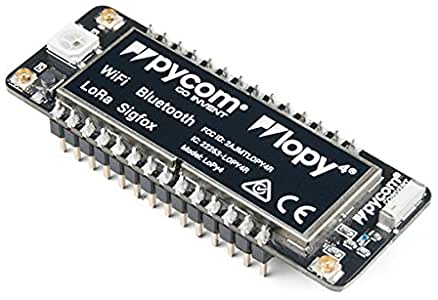
\includegraphics[width=.1\textwidth]{Pictures/LoPy.jpg}};
\node[inner sep=0pt] (RGW) at (3,0) {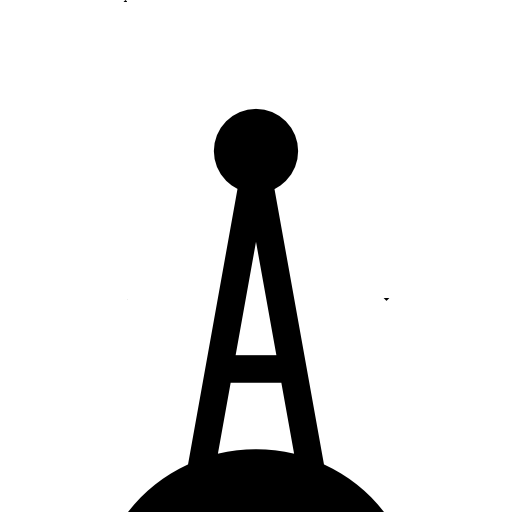
\includegraphics[width=.1\textwidth]{Pictures/antenna.png}};

\draw (5, 0) node (NGW) [cloud, draw] {LNS};

\node[inner sep=0pt] (NAT) at (8,0) {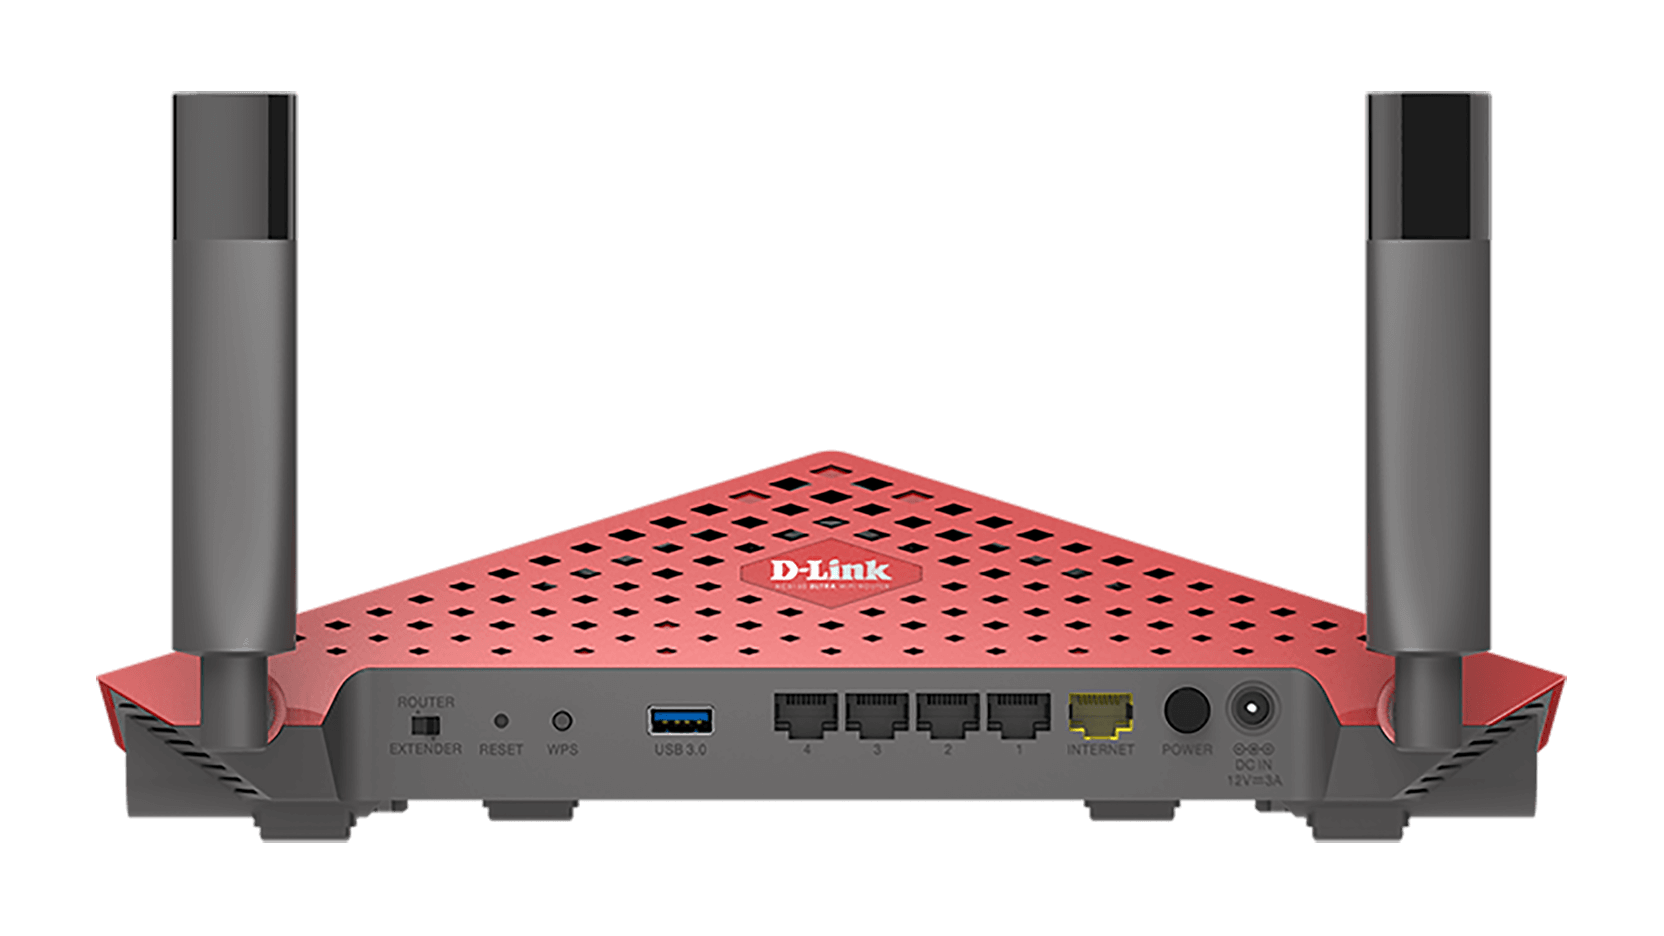
\includegraphics[width=.1\textwidth]{Pictures/router.png}};

\draw (NAT) node [below=15pt] {\small{NAT}};

\draw (12, 0) node (computer) [rectangle, dotted,draw, minimum width=5cm, minimum height=2cm] {};

\draw (10.7, 0) node (relay) [ellipse, dashed, draw, minimum width=2cm, minimum height=1cm] {};
\draw (13.3, 0) node (prog) [ellipse, dashed, draw, minimum width=2cm, minimum height=1cm] {};

\draw (relay) node {\tiny{\texttt{generic\_relay.py}}};
\draw (prog) node {\tiny{\textit{Programme}}};


\draw (12, 0) node [rotate=90] (interface) {\tiny{loopback}};

\draw (computer.north) node [above] {\tiny{Ordinateur}};

\path (lopy) -- +(0, -1.5) coordinate(sline);

\foreach \l in {lopy, RGW, NGW, NAT, relay, prog} {
    \draw [dotted, thin, ->] (\l |- sline) -- +(0, -10); 
}

\path(sline) -- +(0, -0.5) coordinate (a);

\draw (a) node [left, rectangle, draw] {\tiny{msg}};


\draw [decoration={expanding waves,angle=2,segment length=1mm},decorate] (a) -- ([yshift=-0.2cm]a -| RGW) coordinate(b);

\draw [->,decorate,decoration=snake] (b) -- node [above, sloped]{\tiny{packet forwarder}}([yshift=-0.2cm]b -| NGW) coordinate(c); 

\draw [double, double distance=5pt,  green] (c) -- node [above, sloped]{\tiny{POST}} ([yshift=-0.3cm]c -| NAT) coordinate (d); 
\draw [double, double distance=5pt,  orange, ->] (d) --  node [above, sloped]{\tiny{POST}}  ([yshift=-0.3cm]d -| relay) coordinate (e); 
\draw [double, double distance=3pt,  blue] (e) --  node [above, sloped]{\tiny{UDP/IP}}  ([yshift=-0.3cm]e -| prog) coordinate (f); 


\draw (f) node [right, rectangle, draw] {\tiny{msg}};

\draw [thick]  (e) --node [right, near end] {\tiny{Temporisateur}} +(0, -1.5) coordinate (m) ; 

\draw [very thick, orange] (m) -- node [above, sloped]{\tiny{200 OK}}   ([yshift=-0.3cm]m -| NAT) coordinate (n);
\draw [very thick, green, ->] (n) --   node [above, sloped]{\tiny{200 OK}} ([yshift=-0.3cm]n -| NGW) coordinate (o);



% =======
\path(sline) -- +(0, -5) coordinate (a);

\draw (a) node [left, rectangle, draw] {\tiny{msg}};


\draw [decoration={expanding waves,angle=2,segment length=1mm},decorate] (a) -- ([yshift=-0.2cm]a -| RGW) coordinate(b);

\draw [->,decorate,decoration=snake] (b) -- ([yshift=-0.2cm]b -| NGW) coordinate(c); 

\draw [double, double distance=5pt,  green] (c) -- node [above, sloped]{\tiny{POST}} ([yshift=-0.3cm]c -| NAT) coordinate (d); 
\draw [double, double distance=5pt,  orange, ->] (d) --  node [above, sloped]{\tiny{POST}}  ([yshift=-0.3cm]d -| relay) coordinate (e); 
\draw [double, double distance=3pt,  blue] (e) --  node [above, sloped]{\tiny{UDP/IP}}  ([yshift=-0.3cm]e -| prog) coordinate (f); 

\draw (f) node [above right, rectangle, draw] {\tiny{msg}};
\draw (f) node [below right, rectangle, draw] {\tiny{resp}};

\draw [double, double distance=3pt,  blue] (f) --  ([yshift=-0.3cm]f -| relay) coordinate (m); 



\draw [double, double distance=5pt, orange,] (m) -- node [above, sloped]{\tiny{POST}}   ([yshift=-0.3cm]m -| NAT) coordinate (n);
\draw [double, double distance=5pt, green, ->] (n) --   node [above, sloped]{\tiny{POST}} ([yshift=-0.3cm]n -| NGW) coordinate (o);

\draw [thick, -*]  (e) -- (m) coordinate (m) ; 

\draw [very thick, green] (o) --   ([yshift=-0.3cm]o -| NAT) coordinate (s);
\draw [very thick, orange, ->] (s) --   node [above, sloped]{\tiny{200 OK}} ([yshift=-0.3cm]s -| relay) coordinate (t);


\path (t) -- +(0, -0.2) coordinate(w);
\draw [very thick, orange] (w) -- node [above, sloped]{\tiny{200 OK}}   ([yshift=-0.3cm]w -| NAT) coordinate (u);
\draw [very thick, green, ->] (u) --   node [above, sloped]{\tiny{200 OK}} ([yshift=-0.3cm]u -| NGW) coordinate (v);


\draw [dashed, orange] (e) to[bend left] (w);

\path (o) -- +(0, -2) coordinate(p);

\draw [->,decorate,decoration=snake] (p) -- ([yshift=-0.2cm]p -| RGW) coordinate(q); 

\draw [decoration={expanding waves,angle=2,segment length=1mm},decorate] (q) -- ([yshift=-0.2cm]q -| lopy) coordinate(r);

\draw (r) node [left, rectangle, draw] {\tiny{resp}};

\end{tikzpicture}

\caption{Diagramme temporel des échanges.}
\label{fig-ttn-exchanges}
\end{figure}

\section{Thermomètre LoRaWAN}

Le programme \lprog{lorawan\_temperature.py}{pycom} combine la manière de rejoindre le réseau LoRaWAN que l'on à vu précédemment et la partie envoie des séries temporelles différentielles des mesures de température. La seule difficulté réside dans la taille de cette série temporelle. En effet, suivant le \Index{Data Rate} le volume de données transportées diffère. Le tableau~\vref{tab-data-rate} donne la correspondance entre le \textit{Data Rate} et les autres paramètres physique. Il indique également la taille maximales des données transportées.

         \vspace{1em}

Ce changement de taille peut poser des problèmes de compatibilités, si l'on choisi une taille trop grande pour être transmise. En théorie, l'on connaît le \textit{Data Rate} choisi et on peut adapter la taille en conséquence, mais l'opérateur peut aussi modifier le \textit{Data Rate} de l'Objet en fonction des conditions de transmission, et il n'existe aucune instruction en micro-python pour récupérer le \textit{Data Rate} réellement utilisé. Pour simplifier la mise en œuvre, la taille maximale de 50 octets a été choisie. 

\begin{table}
\begin{center}
\begin{tabular}{|c||c|c||c|}
\hline
 \rowcolor{purple!10} Data Rate & Spreading Factor & Largeur de bande & Taille Maximum (octets) \\ \hline \hline
 DR0 & SF12 & 125 KHz & 51 \\ \hline
 DR1 & SF11 & 125 KHz & 51 \\ \hline
 DR2 & SF10 & 125 KHz & 51 \\ \hline
 DR3 & SF9 & 125 KHz & 115 \\ \hline
 DR4 & SF8 & 125 KHz & 242 \\ \hline
 DR5 & SF7 & 125 KHz & 242 \\ \hline
 DR6 & SF7 & 250 KHz & 242 \\ \hline
\end{tabular}
\end{center}
\caption{Data Rate en Europe}
\label{tab-data-rate}
\end{table}


Il suffit de remplacer \pprog{display\_receive\_and\_send.py}{plido-tp3} par \pprog{display\_server.py}{plido-tp3} pour que la série temporelle soit traitée et le résultat envoyé à Beebotte.

\Question{US902}
{En vous aidant du lien suivant \url{https://www.thethingsnetwork.org/docs/lorawan/regional-parameters/} indiquant les paramètres régionaux. Est ce que le programme \lprog{lorawan\_temperature.py}{pycom} fonctionnerait sur un réseau LoRaWAN situé en Amérique du Nord~?}
{Non, la taille maximale des données pour DR0 est de 11 octets.}
\Input{Part10.0-CoAP}
\Input{Part10.5-aiocoap}
\Input{Part11.0-LwM2M}






%%%%%%%%%%%%%%%%%%%%%%%%%%%%%%%%%%%%%



\immediate\closeout\tempfile
\setboolean{Response}{false}

\cleardoublepage
\lgf{\chapter{Réponses aux questions}}
\lge{\chapter{Answers to the questions}}
\input{questions}

\cleardoublepage
\printindex

\cleardoublepage
\printbibliography

\end{document}